\documentclass[9pt]{beamer}
\usetheme{cmepda}

\usepackage[utf8]{inputenc}
\usepackage[T1]{fontenc}


\title{Algorithms and data structures}
\subtitle{Computing Methods for Experimental Physics and Data Analysis}
\date{Compiled on \today}
\author{L. Baldini}
\institute[UNIPI and INFN]{Universit\`a and INFN--Pisa}
\email{luca.baldini@pi.infn.it}


\begin{document}

\titleframe


\begin{frame}
  \frametitle{What is an algorithm?}
  \begin{itemize}
  \item \alert{Algorithm}: a sequence of instructions to perform a computation
  \item Algorithms can be expressed in several different ways
    \begin{itemize}
    \item Flowcarts
    \item Pseudo-code
    \item Working code snippets
    \end{itemize}
  \item The sequence of operation must be expressed unambigously
  \item \alert{Using the right algorithm sometimes makes all the difference
    between being able to attack a problem in a practical time or not}
  \end{itemize}
\end{frame}

\begin{frame}
  \frametitle{Example: sequential vs. binary search}
  \centering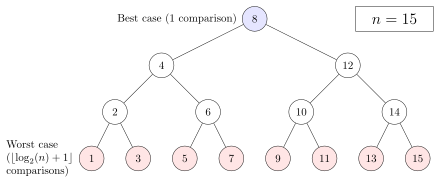
\includegraphics[width=0.6\textwidth]{binary_search}

  \bigskip

  \begin{itemize}
  \item Problem: find an element in a sorted list
  \item \alert{Brute force}: loop over the list until you find (or not) the
    target
  \item \alert{Binary search}
    \begin{itemize}
    \item Start from the middle (if that's the target you're done)
    \item If the target is smaller (larger) than the element in the center,
      bisect the half-list on the left (right)
    \item Iterate until you've found the target (or exhausted the list)
    \end{itemize}
  \item Which algorithm is more efficient?
  \item (This problem is germane to that of finding a person on the phonebook)
  \end{itemize}
\end{frame}


\begin{frame}
  \frametitle{Complexity of an algorithm}
  \begin{Verbatim}[label=\makebox{\url{https://github.com/lucabaldini/cmepda/tree/master/slides/latex/snippets/find\_max.py}},commandchars=\\\{\}]
\PY{k}{def} \PY{n+nf}{find\PYZus{}maximum}\PY{p}{(}\PY{n}{list\PYZus{}}\PY{p}{)}\PY{p}{:}
    \PY{l+s+sd}{\PYZdq{}\PYZdq{}\PYZdq{}Find the biggest element in a list.}
\PY{l+s+sd}{    \PYZdq{}\PYZdq{}\PYZdq{}}
    \PY{n}{maximum} \PY{o}{=} \PY{n}{list\PYZus{}}\PY{p}{[}\PY{l+m+mi}{0}\PY{p}{]}
    \PY{k}{for} \PY{n}{value} \PY{o+ow}{in} \PY{n}{list\PYZus{}}\PY{p}{[}\PY{l+m+mi}{1}\PY{p}{:}\PY{p}{]}\PY{p}{:}
        \PY{k}{if} \PY{n}{value} \PY{o}{\PYZgt{}} \PY{n}{maximum}\PY{p}{:}
            \PY{n}{maximum} \PY{o}{=} \PY{n}{value}
    \PY{k}{return} \PY{n}{maximum}

\PY{n}{l} \PY{o}{=} \PY{p}{[}\PY{l+m+mi}{1}\PY{p}{,} \PY{l+m+mi}{2}\PY{p}{,} \PY{l+m+mi}{5}\PY{p}{,} \PY{l+m+mi}{98}\PY{p}{,} \PY{l+m+mi}{3}\PY{p}{,} \PY{l+m+mi}{1672}\PY{p}{,} \PY{l+m+mi}{6}\PY{p}{,} \PY{l+m+mi}{34}\PY{p}{,} \PY{l+m+mi}{651}\PY{p}{]}
\PY{k}{print}\PY{p}{(}\PY{n}{find\PYZus{}maximum}\PY{p}{(}\PY{n}{l}\PY{p}{)}\PY{p}{)}

[Output]
1672
\end{Verbatim}

  \begin{itemize}
  \item Example: find the largest element in a list of length $n$
  \item How many fundamental instructions is this code executing?
    \begin{itemize}
    \item \alert{(You should realize this is an ill-posed question)}
    \item One assignment and one list lookup at the beginning: $2$
    \item One lookup, one assignment and one comparison for each iteration
      in the for loop: $3(n - 1)$
    \item A variable number of assignments: between $0$ and $(n - 1)$
    \item One final return instruction: 1
    \end{itemize}
  \item \alert{Answer: anything between $3n$ and $4n - 1$}
    \begin{itemize}
    \item (Depending on the input list)
    \end{itemize}
  \end{itemize}
\end{frame}


\begin{frame}
  \frametitle{Complexity of an algorithm}
  \framesubtitle{Continued}
  \begin{itemize}
  \item Message \#1: \alert{the exact number of fundamental instructions that an
    algorithm performs is not determined a priori}
    \begin{itemize}
    \item It depends on the input data, instead
    \item And so does the running time
    \end{itemize}
  \item There's a few questions that you can legitimetely ask, anyway
    \begin{itemize}
    \item How many instructions in the \alert{worst case}?
    \item How many instructions in the \alert{best case}?
    \item How many instructions on \alert{average}?
    \end{itemize}
  \item Message \#2: \alert{the \emph{exact} number of operations doesn't really
    matter}, does it?
    \begin{itemize}
    \item Different machines have different executions speed
    \item Different languages have different meaning of
      \emph{fundamental instruction}
    \end{itemize}
  \item Message \#3: still, \alert{the running time is related to the number
  of fundamental instructions}
  \end{itemize}
\end{frame}


\begin{frame}
  \frametitle{Asymptotic behavior and big-O notation}
  \begin{itemize}
  \item Say you have an algorithm operating on an input of lenght $n$
    \begin{itemize}
    \item e.g., a list with $n$ elements
    \item or a string with $n$ characters 
    \end{itemize}
  \item How many fundamental instructions $N$ does it take to for your algorithm
    to run?
    $$
    N = f(n)
    $$
  \item \alert{Asymptotic behavior}: drop all the terms that grow slowly with
    $n$ and only keep the one that grows faster
    $$
    4n - 1 \approx 4n \quad\text{and}\quad 2n^2 + 6n + 3 \approx 2n^2
    $$
    (for large $n$)
  \item Let's go one step further, and say that we neglect the multiplicative
    factor in front of the leading term
    $$
    4n - 1 \approx n \quad\text{and}\quad 2n^2 + 6n + 3 \approx n^2
    $$
  \item \alert{big-O notation}: the two algorithms are $O(n)$ and $O(n^2)$
  \end{itemize}
\end{frame}


\begin{frame}
  \frametitle{Asymptotic behavior}
  \framesubtitle{Does it matter?}
  \centering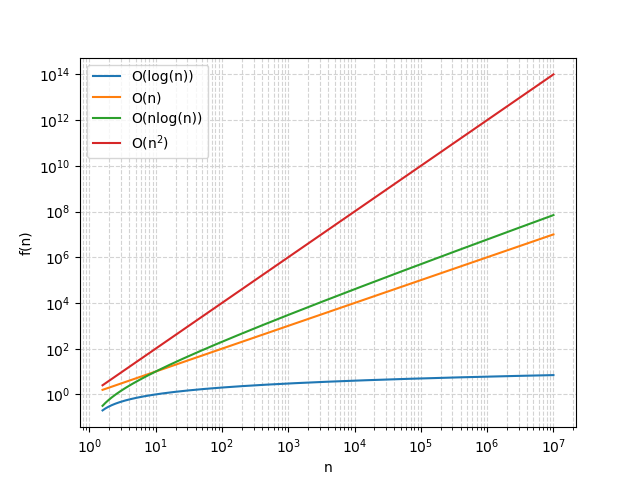
\includegraphics[width=0.75\textwidth]{bigo}

  \begin{itemize}
  \item Yes! If $n = 10^6$ and you can beat down the complexity from $n^2$ to
    $n\log(n)$ you are cutting down the execution time by one million!
  \end{itemize}
\end{frame}


\begin{frame}
  \frametitle{Asymptotic behavior}
  \framesubtitle{How do I measure it?}
  \begin{itemize}
  \item By brute force
    \begin{itemize}
    \item Implement the algorithm
    \item Run it on input data of different size and time the run
    \item (Be careful: results may vary from run to run)
    \item Plot the running time vs. input size
    \end{itemize}
  \item By analysis
    \begin{itemize}
    \item Go ahead and count the instructions
    \item Evaluate the best, worst and average case
    \item (This can be difficult for complex programs, and subject to the
      hidiosyncrasis of the language)
    \end{itemize}
  \item By eye
    \begin{itemize}
    \item One loop: $O(n)$
    \item Two sequential loops: $O(n)$
    \item Two nested loops: $O(n^2)$
    \end{itemize}
  \end{itemize}
\end{frame}


\begin{frame}
  \frametitle{A refreshing reading}
  \framesubtitle{\url{http://www.cs.bme.hu/~friedl/alg/knuth_song_complexity.pdf}}
  \centering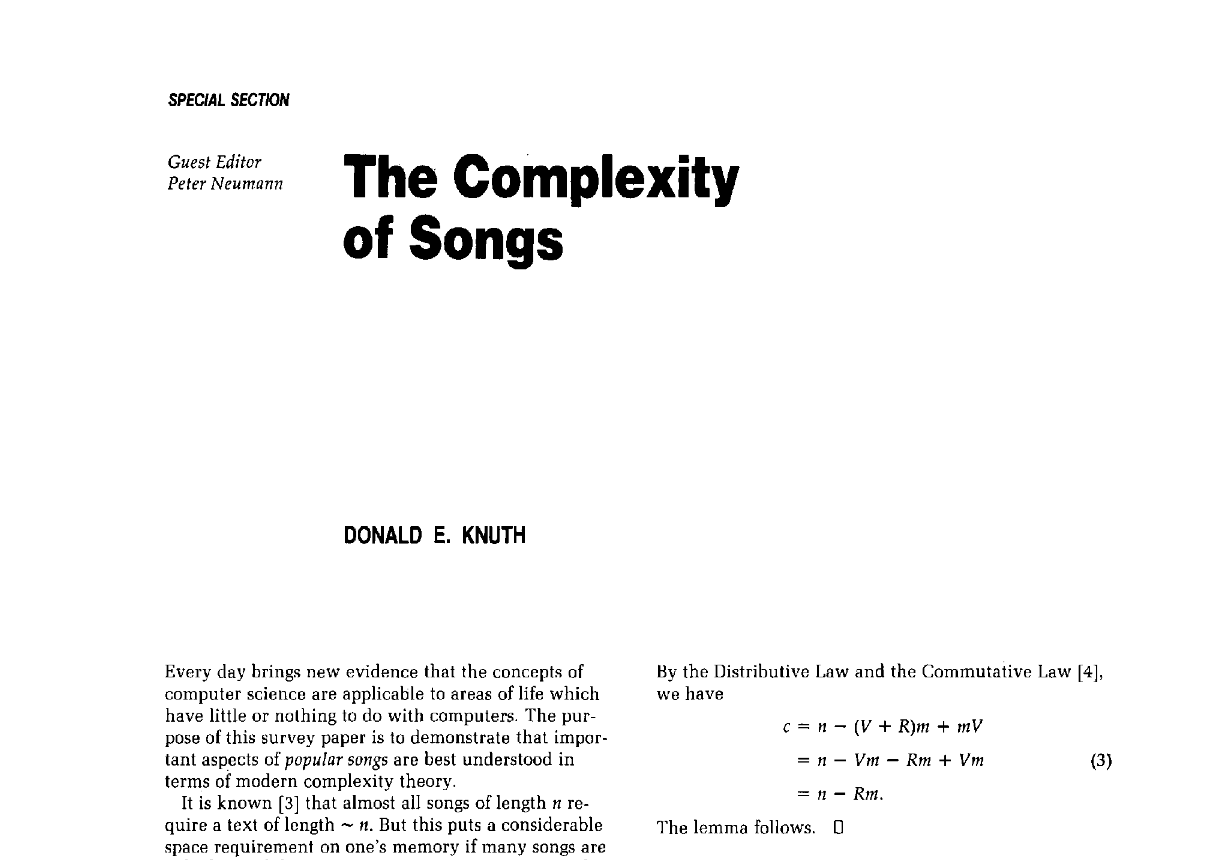
\includegraphics[width=\textwidth]{cos}
\end{frame}


\begin{frame}
  \frametitle{Data structures}
  \framesubtitle{Lists}
  \centering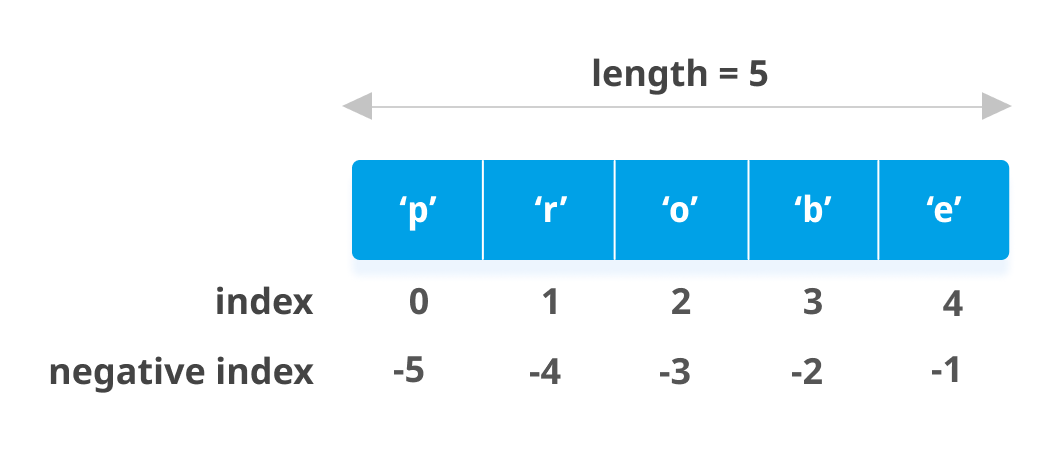
\includegraphics[width=0.6\textwidth]{python-list}

  \bigskip

  \begin{tabular}{lll}
    \hline
    Operation & Average case & Worst case\\
    \hline
    \hline
    Copy & O(n) & O(n)\\
    Append & O(1) & O(1)\\
    Insert & O(n) & O(n)\\
    Get Item & O(1) & O(1)\\
    Set Item & O(1) & O(1)\\
    Delete Item & O(n) & O(n)\\
    Iteration & O(n) & O(n)\\
    min(s), max(s) & O(n) & \\
    Get Length & O(1) & O(1)\\
    \hline
  \end{tabular}
\end{frame}


\begin{frame}
  \frametitle{Hash tables}
  \framesubtitle{Why do I even bring this up? Python dictionaries are hash tables}
  \centering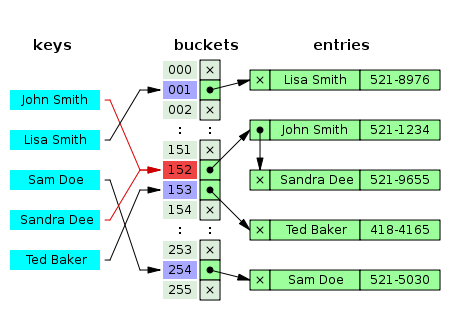
\includegraphics[width=0.6\textwidth]{hash_table}

  \begin{itemize}
  \item Associative array mapping keys to values
  \item Basic idea:
    \begin{itemize}
    \item Pre-allocate some space (which might grow or shrink)
    \item Keys are mapped to indices via a hash function
    \item This is about it, except that you have to be able to handle collisions
    \end{itemize}
  \item Hash tables (aka dictionaries) are highly optimized in Python
  \end{itemize}
\end{frame}


\begin{frame}
  \frametitle{Data structures}
  \framesubtitle{Dictionaries}
  \centering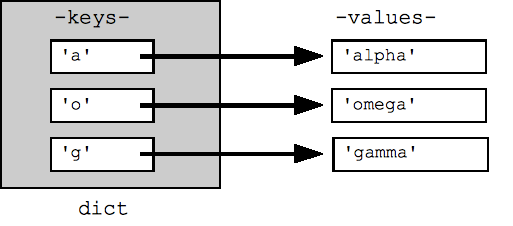
\includegraphics[width=0.6\textwidth]{python-dict}

  \bigskip

  \begin{tabular}{lll}
    \hline
    Operation & Average case & Worst case\\
    \hline
    \hline
    Copy & O(n) & O(n)\\
    Get Item & O(1) & O(n)\\
    Set Item & O(1) & O(n)\\
    Delete Item & O(1) & O(n)\\
    Iteration & O(n) & O(n)\\
    \hline
  \end{tabular}
\end{frame}


\begin{frame}
  \frametitle{An odd corner of Python dictionaries}
  \begin{Verbatim}[label=\makebox{\url{https://bitbucket.org/lbaldini/programming/src/tip/snippets/dict\_hashing.py}},commandchars=\\\{\}]
\PY{k}{print}\PY{p}{(}\PY{n+nb}{hash}\PY{p}{(}\PY{l+m+mi}{3}\PY{p}{)}\PY{p}{)}
\PY{k}{print}\PY{p}{(}\PY{n+nb}{hash}\PY{p}{(}\PY{l+m+mf}{3.}\PY{p}{)}\PY{p}{)}

\PY{n}{d} \PY{o}{=} \PY{p}{\PYZob{}}\PY{p}{\PYZcb{}}

\PY{n}{d}\PY{p}{[}\PY{l+m+mi}{3}\PY{p}{]} \PY{o}{=} \PY{l+s+s1}{\PYZsq{}}\PY{l+s+s1}{Hi there!}\PY{l+s+s1}{\PYZsq{}}
\PY{k}{print}\PY{p}{(}\PY{n}{d}\PY{p}{)}

\PY{n}{d}\PY{p}{[}\PY{l+m+mf}{3.}\PY{p}{]} \PY{o}{=} \PY{l+s+s1}{\PYZsq{}}\PY{l+s+s1}{How are you?}\PY{l+s+s1}{\PYZsq{}}
\PY{k}{print}\PY{p}{(}\PY{n}{d}\PY{p}{)}

[Output]
3
3
{3: 'Hi there!'}
{3: 'How are you?'}
\end{Verbatim}

  \begin{itemize}
  \item When a float corresponds to an integer, its hash is the same as that
    of the integer
  \item The hash is used to map keys into indices
  \item Therefore: $3$ and $3.$ are the same key to a dictionary
  \end{itemize}
\end{frame}


\begin{frame}
  \frametitle{A real-life example: sorting}
  \begin{Verbatim}[label=\makebox{\url{https://github.com/lucabaldini/cmepda/tree/master/slides/latex/snippets/sloppy\_sort.py}},commandchars=\\\{\}]
\PY{k}{def} \PY{n+nf}{sloppy\PYZus{}sort}\PY{p}{(}\PY{n}{list\PYZus{}}\PY{p}{)}\PY{p}{:}
    \PY{l+s+sd}{\PYZdq{}\PYZdq{}\PYZdq{}Poor man\PYZsq{}s implementation of a sorting algorithm.}
\PY{l+s+sd}{    \PYZdq{}\PYZdq{}\PYZdq{}}
    \PY{n}{sorted\PYZus{}list} \PY{o}{=} \PY{p}{[}\PY{p}{]}
    \PY{k}{for} \PY{n}{item} \PY{o+ow}{in} \PY{n}{list\PYZus{}}\PY{p}{:}
        \PY{k}{if} \PY{n+nb}{len}\PY{p}{(}\PY{n}{sorted\PYZus{}list}\PY{p}{)} \PY{o}{==} \PY{l+m+mi}{0}\PY{p}{:}
            \PY{n}{sorted\PYZus{}list}\PY{o}{.}\PY{n}{append}\PY{p}{(}\PY{n}{item}\PY{p}{)}
        \PY{k}{else}\PY{p}{:}
            \PY{k}{if} \PY{n}{item} \PY{o}{\PYZlt{}} \PY{n}{sorted\PYZus{}list}\PY{p}{[}\PY{l+m+mi}{0}\PY{p}{]}\PY{p}{:}
                \PY{n}{sorted\PYZus{}list}\PY{o}{.}\PY{n}{insert}\PY{p}{(}\PY{l+m+mi}{0}\PY{p}{,} \PY{n}{item}\PY{p}{)}
            \PY{k}{else}\PY{p}{:}
                \PY{k}{for} \PY{n}{i}\PY{p}{,} \PY{n}{sorted\PYZus{}item} \PY{o+ow}{in} \PY{n+nb}{enumerate}\PY{p}{(}\PY{n}{sorted\PYZus{}list}\PY{p}{)}\PY{p}{:}
                    \PY{k}{if} \PY{n}{item} \PY{o}{\PYZlt{}}\PY{o}{=} \PY{n}{sorted\PYZus{}item}\PY{p}{:}
                        \PY{n}{sorted\PYZus{}list}\PY{o}{.}\PY{n}{insert}\PY{p}{(}\PY{n}{i}\PY{p}{,} \PY{n}{item}\PY{p}{)}
                        \PY{k}{break}
    \PY{k}{return} \PY{n}{sorted\PYZus{}list}

\PY{n}{l} \PY{o}{=} \PY{p}{[}\PY{l+m+mi}{10}\PY{p}{,} \PY{l+m+mi}{1}\PY{p}{,} \PY{l+m+mi}{5}\PY{p}{,} \PY{l+m+mi}{2}\PY{p}{,} \PY{l+m+mi}{7}\PY{p}{,} \PY{l+m+mi}{3}\PY{p}{,} \PY{l+m+mi}{9}\PY{p}{,} \PY{l+m+mi}{4}\PY{p}{]}
\PY{k}{print}\PY{p}{(}\PY{n}{l}\PY{p}{)}
\PY{k}{print}\PY{p}{(}\PY{n}{sloppy\PYZus{}sort}\PY{p}{(}\PY{n}{l}\PY{p}{)}\PY{p}{)}

[Output]
[10, 1, 5, 2, 7, 3, 9, 4]
[1, 2, 3, 4, 5, 7, 9, 10]
\end{Verbatim}

  \begin{itemize}
  \item Say you are asked to implement an algorithm to sort a list
    \begin{itemize}
    \item Chances are that you would come up with two nested loops, O($n^2$)
    \end{itemize}
  \end{itemize}
\end{frame}


\begin{frame}
  \frametitle{Sorting algorithms on the market}
  \framesubtitle{aka Don't try this at home}
  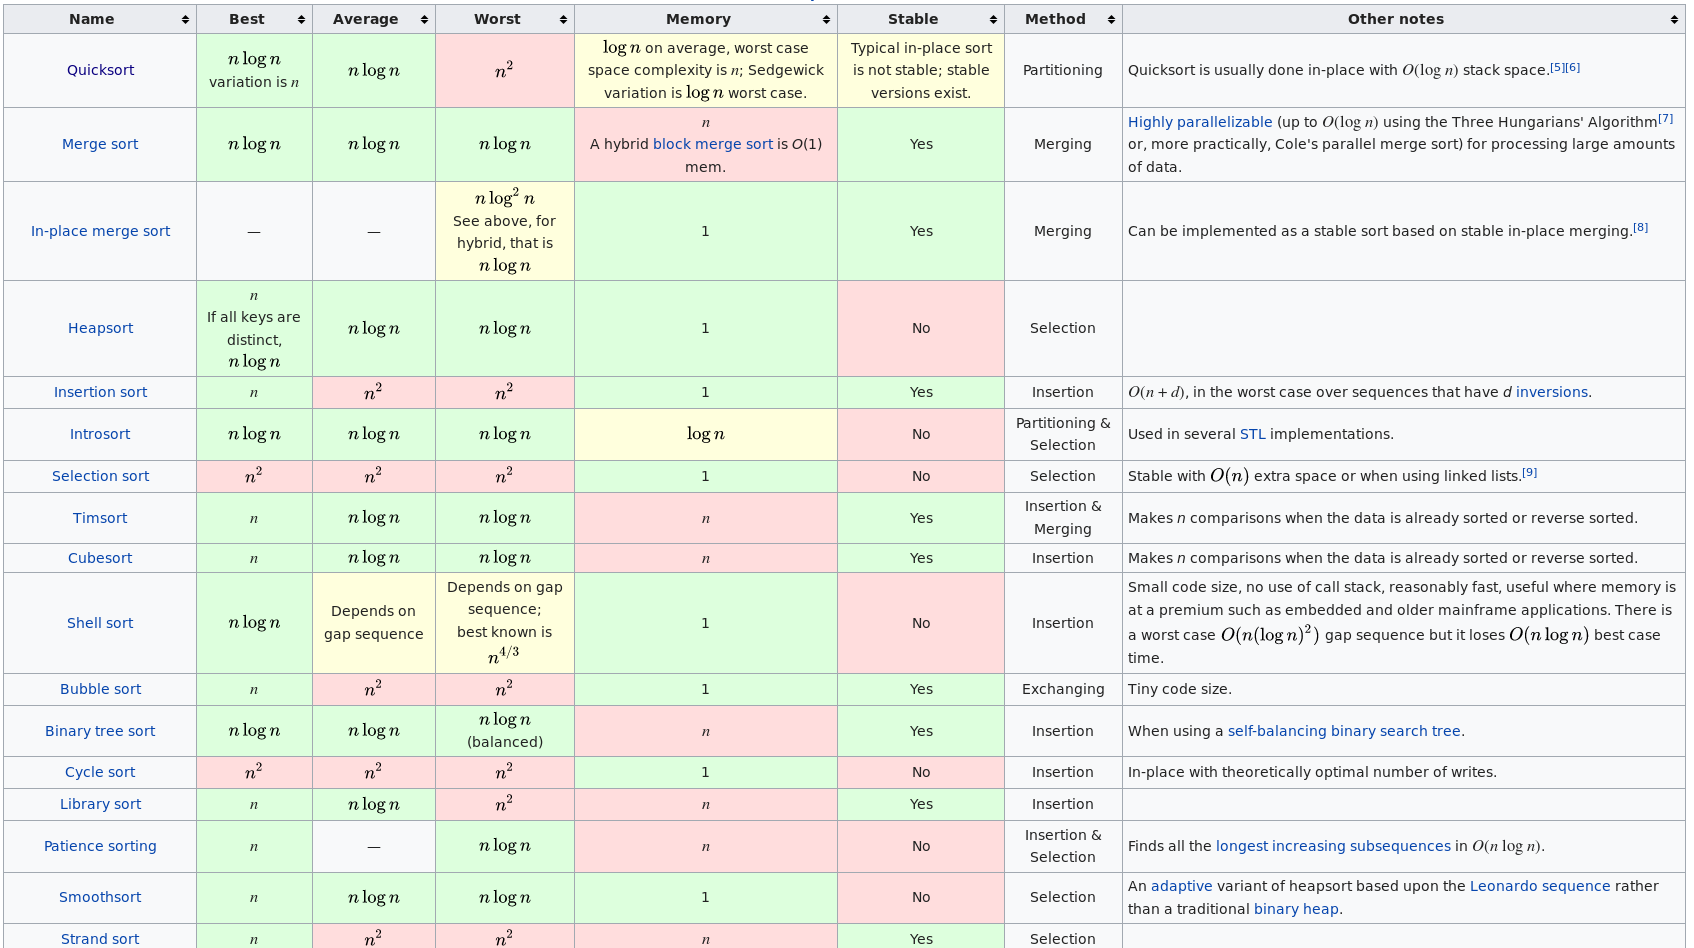
\includegraphics[width=\textwidth]{sorting_algs}
\end{frame}


\begin{frame}
  \frametitle{What is Python using? Timsort}
  \framesubtitle{The name comes from Tim Peters}
  \begin{Verbatim}[label=\makebox{\url{https://github.com/lucabaldini/cmepda/tree/master/slides/latex/snippets/timsort.py}},commandchars=\\\{\}]
\PY{n}{l} \PY{o}{=} \PY{p}{[}\PY{l+m+mi}{10}\PY{p}{,} \PY{l+m+mi}{1}\PY{p}{,} \PY{l+m+mi}{5}\PY{p}{,} \PY{l+m+mi}{2}\PY{p}{,} \PY{l+m+mi}{7}\PY{p}{,} \PY{l+m+mi}{3}\PY{p}{,} \PY{l+m+mi}{9}\PY{p}{,} \PY{l+m+mi}{4}\PY{p}{]}
\PY{k}{print}\PY{p}{(}\PY{n}{l}\PY{p}{)}
\PY{n}{l}\PY{o}{.}\PY{n}{sort}\PY{p}{(}\PY{p}{)}
\PY{k}{print}\PY{p}{(}\PY{n}{l}\PY{p}{)}

[Output]
[10, 1, 5, 2, 7, 3, 9, 4]
[1, 2, 3, 4, 5, 7, 9, 10]
\end{Verbatim}

  \bigskip
  
  \begin{itemize}
  \item Hybrid algorithm, derived from merge sort and insertion sort
    \begin{itemize}
    \item Find subsequences of the data that are already ordered
    \item Use that knowledge to sort the remainder more efficiently
    \end{itemize}
  \item ``Although practicality beats purity'' (The Zen of Python)
  \end{itemize}
\end{frame}


\begin{frame}
  \frametitle{References}
  \scriptsize
  \begin{itemize}
  \item \url{https://en.wikipedia.org/wiki/Algorithm}
  \item \url{https://discrete.gr/complexity/}
  \item \url{https://wiki.python.org/moin/TimeComplexity}
  \item \url{https://en.wikipedia.org/wiki/Sorting_algorithm}
  \item \url{https://bugs.python.org/file4451/timsort.txt}
  \item \url{https://en.wikipedia.org/wiki/Timsort}
  \end{itemize}
\end{frame}



\end{document}
